
\begin{center}
\Large\textbf{MicroBooNE}
\end{center}

The MicroBooNE experiment serves as the first detector deployed at the SBN facility and represents the next step in LArTPC technology. MicroBooNE is a 10.3~m~$\times$~2.5~m~$\times$~2.3~m TPC with 89 tons of active volume. The TPC, shown in Figure \ref{fig:uboone}, has three instrumented wire planes with the first two induction planes oriented at $\pm 30^{\circ}$ to the beam axis and the final plane oriented vertically. Both the pitch and wire spacing is chosen to be 3~mm, which provides superb resolution for imaging interactions inside the detector. Additionally there are 32, 8'' cryogenic photomultiplier tubes (PMTs) which provide the $t_{0}$ for an interaction by recording the scintillation light produced when the charged particles interact in the argon.

\begin{figure}[htb]
\centering
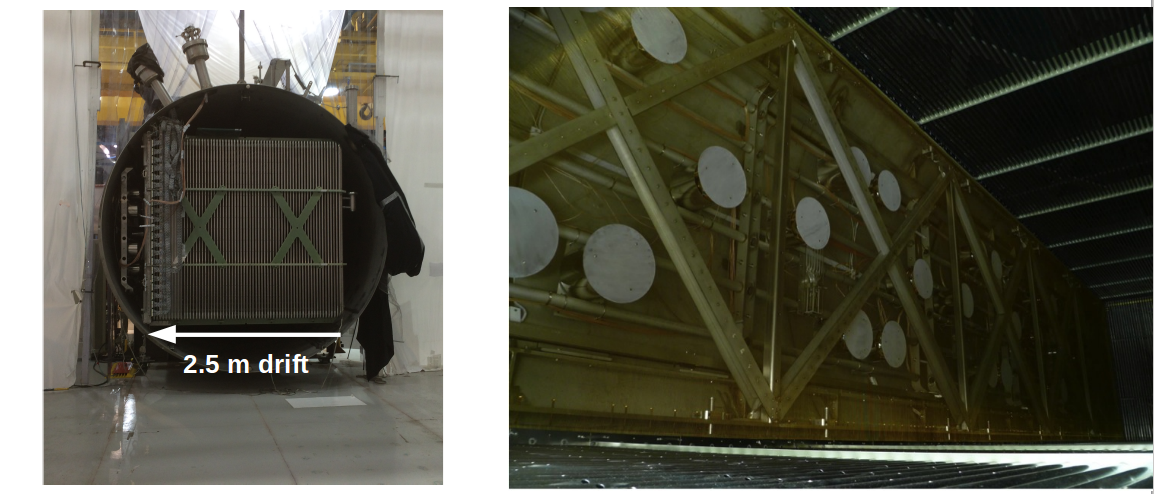
\includegraphics[width=0.85\textwidth]{images/microboone.png}
\caption[]{The MicroBooNE TPC after installation inside the cryostat and a long exposure view of the inside of the TPC. The acrylic disks coated in wavelength shifting material which sit directly in front of the PMTs can be seen behind the wire planes.}
\label{fig:uboone}
\end{figure}

In the summer of 2015 MicroBooNE was filled with liquid argon and began commissioning. During this initial commissioning the drift high voltage was brought to $\sim 45\%$ its nominal value and immediately cosmic ray tracks and scintillation light were able to be seen. Figure \ref{} shows some of the first cosmic ray tracks as seen by the collection plane and the light readout as seen by the PMT system. With the rapid success of the system, MicroBooNE has now transitioned from commissioning to neutrino data taking starting in October of 2015. 

\begin{figure}[htb]
\centering
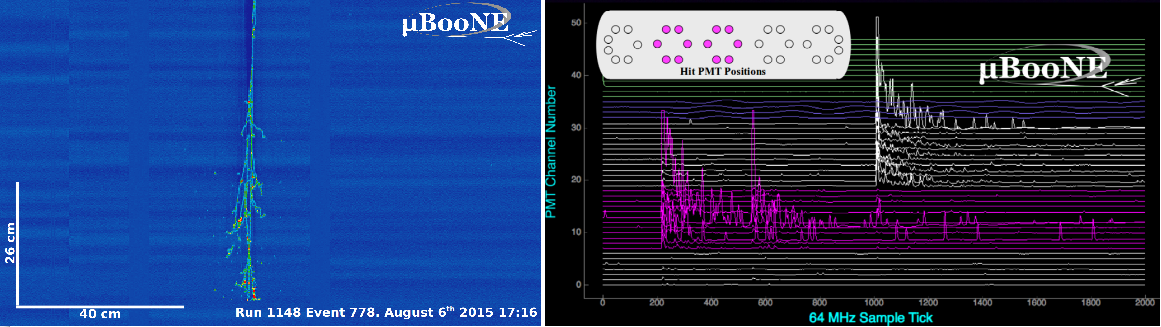
\includegraphics[width=0.98\textwidth]{images/microbooneEvents.png}
\caption[]{MicroBooNE's first cosmic ray events as seen by the TPC collection plane and the PMT readout.}
\label{fig:ubooneEvents}
\end{figure}

One of the most compelling measurements MicroBooNE will make is to confirm or refute the nature of the MiniBooNE low-energy electron neutrino excess. Utilizing the particle identification powers of the LArTPC (specifically the dE/dX discrimination), MicroBooNE will be able to differentiate the electron-like electromagnetic showers from photon-like electromagnetic showers. Moreover, the dominant background in the MiniBooNE analysis of neutral current $\pi^{0}$ production can be eliminated using the powerful imaging techniques of a LArTPC. The analysis techniques developed for the MiniBooNE low energy excess search will be developed in the common software framework known as LArSoft. This software framework is common amongst many of the LArTPC experiments, helping ensure that the reconstruction techniques and analysis strategies developed on MicroBooNE will have applicability to future experiments.

MicroBooNE will also be able to measure many high-statistic cross-sections at $E_{\nu} < 1$GeV. At this energy range, the impact of various nuclear effects such as final state interactions and short-range nucleon correlation are poorly understood. These nuclear effects can change the classification of neutrino nucleus interaction, and thus change the measured cross-section. The fine grain tracking offered by LArTPCs allows for the classification of neutrino-nucleon interaction in terms of final state particles instead of using simplifications such as the quasi-elastic scattering assumption. Moreover, with a proton threshold measured as low as 21~MeV of kinetic energy \cite{Argoneut}, these nuclear effects can event be measured with high statistics using neutrinos as a probe. The broader neutrino cross-section community is anticipating how the results measured by MicroBooNE compare to previous measurements.

MicroBooNE will also explore the physics capabilities of LArTPC including classification of low energy events as a background for supernova neutrinos and searching for cosmogenic backgrounds related to proton decay analysis. While MicroBooNE is too small and located on the surface making meaningful proton decay search impossible. However, utilizing the abundance of cosmic rays to search for background signatures due to cosmogenic sources can provide useful input to future analysis targeted at the Deep Underground Neutrino Experiment (DUNE). Additionally, Prof. Asaadi serves as the convener of the Astro-Particle and Exotics working group on MicroBooNE and is currently leading analyses related to proton decay backgrounds and exotic dark matter searches at a beam dump. Fully exploring the physics capabilities of the MicroBooNE detector enables a robust physics program. 

%%%%%%%%%%%%%%%%%%%%%%%%%%%%%%%%%%%%%%%%%%%%%%%%%%%%%%%%%%%%%%%%%%%%%
\subsubsection{Proposed work on MicroBooNE}\label{sec:proposeUboone}
%%%%%%%%%%%%%%%%%%%%%%%%%%%%%%%%%%%%%%%%%%%%%%%%%%%%%%%%%%%%%%%%%%%%%
UT Arlington will play a major role in the data taking and operations of the MicroBooNE detector. Prof. Asaadi has served as the TPC commissioning leader and is now transitioning to the TPC operations expert. Prof. Asaadi will also continue in his role as Astro-Particle and Exotics working group convener for the foreseeable future where he will continue to shape the early data analyses as well as explore new physics opportunities with the MicroBooNE detector.

The postdoctoral researcher supported by this proposal will spend much of their time working on the MicroBooNE operations and is expected to be trained to serve as the TPC operations expert. In addition to data taking shift requirements, the he/she is also expected to play a role in the online DAQ/data quality management as training for the future planned work on the SBND DAQ. The graduate student supported by this work is also expected to take shifts on MicroBooNE and play a supporting role on the expert training.

Being a driving force on early neutrino cross-section analysis is a good way to have impact on the physics program at MicroBooNE. The postdoctoral researcher and graduate student are expected to work on neutrino cross-section analysis using the data taken in the first year of running. This data set will provide the first high statistics glimpse into the short-baseline analysis. Following up on previous low statistics cross-sections measured by ArgoNeuT including the coherent charged pion production and neutral current $\pi^{0}$ is one way which they can have immediate impact. Furthermore, the tools developed for data analysis and reconstruction in MicroBooNE will have transferability to future LArTPC through the use of the common software package, LArSoft.
Neutrino cross-section analysis
